\documentclass{article}
\usepackage[utf8]{inputenc}
\usepackage{float}
\usepackage[spanish]{babel}
\usepackage{graphicx}
\usepackage{listings}
\usepackage{color}
\usepackage{datetime}
\newdate{date}{12}{02}{2019}

\title{Tarea 1}
\author{Jesus Angel Patlán Castillo (5621)}
\date{\displaydate{date}}



\begin{document}

\definecolor{codegreen}{rgb}{0,0.6,0}
\definecolor{codegray}{rgb}{0.5,0.5,0.5}
\definecolor{codepurple}{rgb}{0.58,0,0.82}
\definecolor{backcolour}{rgb}{0.95,0.95,0.92}
 
\lstdefinestyle{mystyle}{
    backgroundcolor=\color{backcolour},   
    commentstyle=\color{codegreen},
    keywordstyle=\color{magenta},
    numberstyle=\tiny\color{codegray},
    stringstyle=\color{codepurple},
    basicstyle=\footnotesize,
    breakatwhitespace=false,         
    breaklines=true,                 
    captionpos=b,                    
    keepspaces=true,                 
    numbers=left,                    
    numbersep=5pt,                  
    showspaces=false,                
    showstringspaces=false,
    showtabs=false,                  
    tabsize=2
}
 
\lstset{style=mystyle}


\maketitle

En esta tarea se recopila información de grafos con distintas propiedades. Se utiliza código de Python \cite{Python}, con la librería NetworkX \cite{NetworkX} para la generación de grafos y la librería Matplotlib \cite{Matplotlib} para guardar el grafo en el formato ".eps". El código empleado se obtuvo consultando la documentación oficial de la librería NetworkX \cite{NetworkXD} y guías suplementarias \cite{SOQ1} \cite{SOQ2}. Las imágenes y el código se encuentran disponibles directamente en mi repositorio \cite{JAPC}.


\section{Grafo simple no dirigido acíclico}
Una red de ciudades en un estado puede ser un ejemplo de un grafo simple no dirigido acíclico, ya que podemos representar cada ciudad como un nodo del grafo, y tomar en cuenta que cada arista representan las carreteras que conectan cada ciudad, considerando que sería un grafo no dirigido dado que una carretera puede ir de ida y vuelta entre ciudades, y es acíclico puesto que no se consideran carreteras que van de una ciudad a sí misma \cite{novo2004aplicaciones}. La figura \ref{fig:GSNDA} representa un ejemplo de este tipo de grafo.

\begin{figure}[H]
    \includegraphics[width=\textwidth]{1-GSNDA}
    \caption{Grafo simple no dirigido acíclico}
    \label{fig:GSNDA}
\end{figure}


\lstinputlisting[language=Python,firstline=5]{1-GSNDA.py}


\section{Grafo simple no dirigido cíclico}
Una ruta de autobús puede ser representada por este tipo de grafos, en donde los autobuses pasan a través de las calles y avenidas (representadas con las aristas), y cada nodo del grafo se puede representar una parada donde se recogen personas. La figura \ref{fig:GSNDC} representa un ejemplo de este tipo de grafo.
\begin{figure}[H]
    \includegraphics[width=\textwidth]{2-GSNDC}
    \caption{Grafo simple no dirigido cíclico}
    \label{fig:GSNDC}
\end{figure}


\lstinputlisting[language=Python,firstline=5]{2-GSNDC.py}
\section{Grafo simple no dirigido reflexivo}
Podemos representar una red de sistemas informáticos por medio de un grafo reflexivo, donde cada computadora es representada por medio de un nodo, y la conexión hacia las demás computadoras son representadas por las aristas. La arista reflexiva representaría la conexión de una computadora consigo misma \cite{GSNDR}. La figura \ref{fig:GSNDR} representa un ejemplo de este tipo de grafo.
\begin{figure}[H]
    \includegraphics[width=\textwidth]{3-GSNDC}
    \caption{Grafo simple no dirigido reflexivo (El nodo 1 tiene una arista reflexiva)}
    \label{fig:GSNDR}
\end{figure}


\lstinputlisting[language=Python,firstline=5]{3-GSNDR.py}
\section{Grafo simple dirigido acíclico}
En la Programación Orientada a Objetos es común realizar herencia entre clases, y esta puede ser representada por medio de un grafo dirigido acíclico, teniendo a cada nodo como una clase distinta, y señalando la herencia por medio de una arista dirigida a las clases hijas \cite{GSDA}. La figura \ref{fig:GSDA} representa un ejemplo de este tipo de grafo.
\begin{figure}[H]
    \includegraphics[width=\textwidth]{4-GSDA}
    \caption{Grafo simple dirigido acíclico}
    \label{fig:GSDA}
\end{figure}


\lstinputlisting[language=Python,firstline=5]{4-GSDA.py}
\section{Grafo simple dirigido cíclico}
En algunos juegos se tienen distintos estados en los que el jugador se puede encontrar, y esto puede ser representado en un grafo dirigido cíclico, dado que cada estado se puede visualizar por medio de un nodo, y las aristas representarían las maneras en las que un estado puede cambiar a otro \cite{GSDA}. La figura \ref{fig:GSDC} representa un ejemplo de este tipo de grafo.
\begin{figure}[H]
    \includegraphics[width=\textwidth]{5-GSDC}
    \caption{Grafo simple dirigido cíclico}
    \label{fig:GSDC}
\end{figure}


\lstinputlisting[language=Python,firstline=5]{5-GSDC.py}
\section{Grafo simple dirigido reflexivo}
Se  puede realizar un grafo dirigido reflexivo para representar todos los hipervínculos (aristas) que dirigen a una página web (nodos) en los que el usuario puede navegar a través de una web, cuando una página web se redirige a sí misma se utiliza una arista reflexiva \cite{GSDA}. La figura \ref{fig:GSDR} representa un ejemplo de este tipo de grafo.
\begin{figure}[H]
    \includegraphics[width=\textwidth]{6-GSDR}
    \caption{Grafo simple dirigido reflexivo (El nodo 1 tiene una arista reflexiva)}
    \label{fig:GSDR}
\end{figure}


\lstinputlisting[language=Python,firstline=5]{6-GSDR.py}
\section{Multigrafo no dirigido acíclico}
De manera similar al ejemplo de un grafo simple no dirigido acíclico, una red de ciudades puede ser representado por un multigrafo, el cual puede proporcionar más información que un grafo simple al añadir diversos caminos por el que se puede trasladar de un nodo a otro. La figura \ref{fig:MNDA} representa un ejemplo de este tipo de grafo.
\begin{figure}[H]
    \includegraphics[width=\textwidth]{7-MNDA}
    \caption{Multigrafo no dirigido acíclico (Los nodos 1 y 2 tienen múltiples aristas)}
    \label{fig:MNDA}
\end{figure}


\lstinputlisting[language=Python,firstline=5]{7-MNDA.py}
\section{Multigrafo no dirigido cíclico}
Considerando el ejemplo de la ruta de autobuses, podemos tener entre dos paradas (nodos) múltiples rutas para llegar a la parada siguiente. La figura \ref{fig:MNDC} representa un ejemplo de este tipo de grafo.
\begin{figure}[H]
    \includegraphics[width=\textwidth]{8-MNDC}
    \caption{Multigrafo no dirigido cíclico (Los nodos 1, 2 y 3 tienen múltiples aristas)}
    \label{fig:MNDC}
\end{figure}


\lstinputlisting[language=Python,firstline=5]{8-MNDC.py}
\section{Multigrafo no dirigido reflexivo}
En las redes sociales, se puede utilizar un multigrafo reflexivo para representar las menciones que se hacen entre usuarios por medio de publicaciones, donde cada nodo representa un usuario y cada publicación representa la arista con la que conecta el usuario que realizo la publicación con el que es mencionado. La figura \ref{fig:MNDR} representa un ejemplo de este tipo de grafo.

\begin{figure}[H]
    \includegraphics[width=\textwidth]{9-MNDR}
    \caption{Multigrafo no dirigido reflexivo (Los nodos 1 y 2 tienen múltiples aristas, el nodo 1 tiene una arista reflexiva)}
    \label{fig:MNDR}
\end{figure}


\lstinputlisting[language=Python,firstline=5]{9-MNDR.py}
\section{Multigrafo dirigido acíclico}
Con un multigrafo dirigido acíclico es posible representar el flujo de dinero entre cuentas bancarias, tomando las cuentas bancarias como los nodos del grafo y las aristas el método de traspaso de una cuenta a otra. La figura \ref{fig:MDA} representa un ejemplo de este tipo de grafo.
\begin{figure}[H]
    \includegraphics[width=\textwidth]{10-MDA}
    \caption{Multigrafo dirigido acíclico (Los nodos 1 y 4 tienen múltiples aristas)}
    \label{fig:MDA}
\end{figure}


\lstinputlisting[language=Python,firstline=5]{10-MDA.py}
\section{Multigrafo dirigido cíclico}
Tomando el ejemplo utilizado en los grafos simples dirigidos cíclicos, en los juegos es posible que haya diferentes maneras de pasar de un estado a otro, lo cual es representado por aristas múltiples entre los nodos. La figura \ref{fig:MDC} representa un ejemplo de este tipo de grafo.
\begin{figure}[H]
    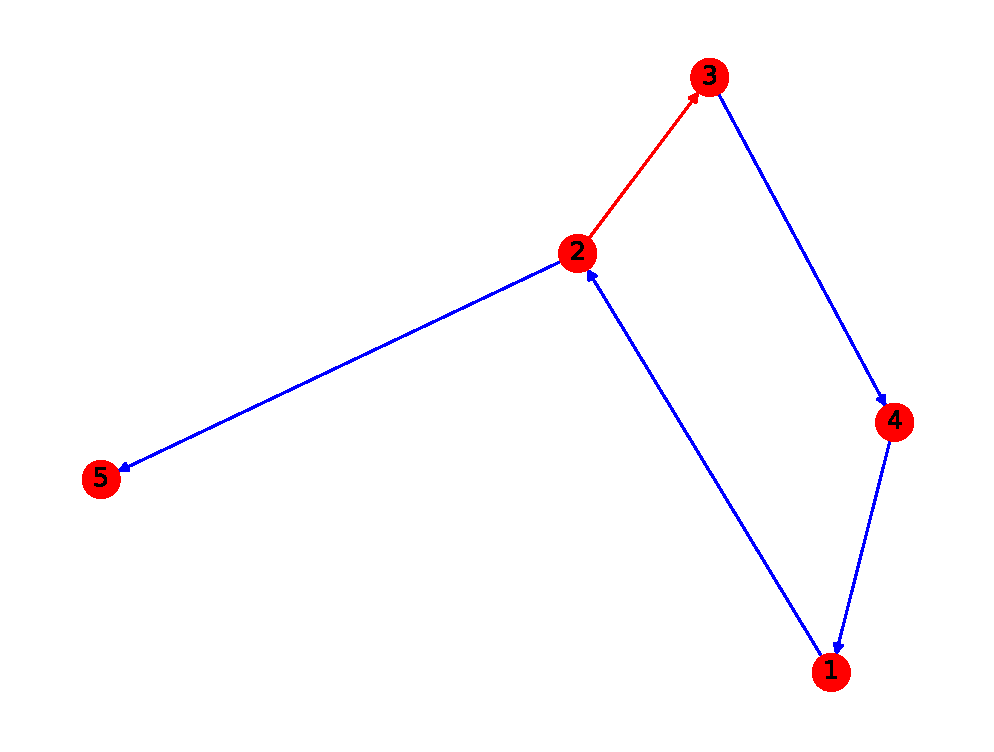
\includegraphics[width=\textwidth]{11-MDC}
    \caption{Multigrafo dirigido cíclico (Los nodos 2 y 3 tienen múltiples aristas)}
    \label{fig:MDC}
\end{figure}


\lstinputlisting[language=Python,firstline=5]{11-MDC.py}
\section{Multigrafo dirigido reflexivo}
Como en el grafo simple dirigido reflexivo, en una página web se pueden tener múltiples hipervínculos que te redirigen a una misma página web. La figura \ref{fig:MDR} representa un ejemplo de este tipo de grafo.
\begin{figure}[H]
    \includegraphics[width=\textwidth]{12-MDR}
    \caption{Multigrafo dirigido reflexivo (Los nodos 3 y 4 tienen múltiples aristas, el nodo 1 tiene una arista reflexiva)}
    \label{fig:MDR}
\end{figure}


\lstinputlisting[language=Python,firstline=5]{12-MDR.py}




\bibliographystyle{plain}
\bibliography{references}

\end{document}
